% You should title the file with a .tex extension (hw1.tex, for example)
\documentclass[a4paper, 12pt]{report}

\usepackage{mathtools}
\usepackage{amsmath}
\usepackage{amssymb}
\usepackage{tabularx}
\usepackage{fancyhdr}
\usepackage{minted}
\usepackage{amsthm}        
\usepackage{graphicx}
\usepackage{algorithm}
\usepackage{algpseudocode}
\usepackage{natbib}
\usepackage{hyperref}
\hypersetup{
    colorlinks=true,
    linkcolor=black,
    filecolor=magenta,      
    urlcolor=cyan,
    pdfborder=white,
    citecolor=black,
    pdfpagemode=FullScreen,
}

\renewcommand{\bibsection}{\chapter*{Reference}}

\newcommand{\remark}[3]{%
    {\colorbox{#2}{\sffamily\scriptsize\bfseries\textcolor{white}{#1}}}
    {\textbf{\textcolor{#2}{#3}}}
}

\renewcommand\qedsymbol{$\blacksquare$}

\DeclarePairedDelimiter\ceil{\lceil}{\rceil}
\DeclarePairedDelimiter\floor{\lfloor}{\rfloor}


\graphicspath{ {./pictures} }

\usepackage[margin=1in]{geometry}

\newcommand{\question}[2] {\vspace{.25in} \hrule\vspace{0.5em}
\noindent{\bf #1: #2} \vspace{0.5em}
\hrule \vspace{.10in}}
\renewcommand{\part}[1] {\vspace{.10in} {\bf (#1)}}

\newcommand{\myname}{P. Archer, N. Krittin}
\newcommand{\mySubject}{ICCS315 Applied Algorithms}

\setlength{\parindent}{20pt}
\setlength{\parskip}{5pt plus 1pt}
 
\pagestyle{fancyplain}
\lhead{\fancyplain{}{\textbf{False Sharing}}}      % Note the different brackets!
\rhead{\fancyplain{}{\myname}}
\chead{\fancyplain{}{\mySubject}}

\title{

	{
\includegraphics[width=80mm,scale=0.5]{MUIC_Logo_Eng_Center.png}} \\
	{\textbf{\mySubject}}\\
	{\large False Sharing}\\
}
\author{
	{\textbf{Written by}} \\ 
	{Archer N. Phillips 6280562, Krittin Nisunarat 6280782} \\
}
\date{9 April 2023}
\thispagestyle{plain}


\begin{document}
\maketitle
\begin{abstract}
	\par We can not deny that cache protocols are essential for improving the performance of computer systems in several ways. One essential way is by reducing 
the time it takes to access data from memory. However, the restriction is the size of it with a tread off.
Obviously, any kinds of volatile memories have a small size, but fast storage area that stores frequently used data and instructions so that they can be 
accessed quickly by the processor. However, the performance is uncertain as some data can be stored on the same address on share stage cache line.
This situation is well-known in computer science that is called \textbf{false sharing}.

\par False sharing is essentially a performance-degrading usage pattern  that can arise in systems with distributed, coherent caches at the size of the smallest 
resource block managed by the caching mechanism When a system participant attempts to periodically access data that is not being altered by another party, but that 
data shares a cache block with data that is being altered, the caching protocol may force the first participant to reload the whole cache block despite a lack of logical necessity.
The caching system is unaware of activity within this block and forces the first participant to bear the caching system overhead required by true shared access of a resource.
This can happen several ways which will be discussed in this paper after the experiment.

In this paper, MESIF cache coherence protocol will be discussed in detail and stage management of the cache protocol in multiprocessor.
In addition, existing solution will be illustrated as many of architectures and programming languages are integrated. Finally, our false sharing 
solution will be determined at the end of the paper.
\end{abstract}
\tableofcontents

\chapter{Cache Coherence and its performance}
\section{Understanding of cache coherence in single core}

Before we determine and analyze MESIF protocol, there are a few important concept
about read-write memory transaction in both single core or multiple cores. To understand
coherence, suppose that we are executing a single core algorithm $S$ on x86 machine and the task
that is sent to processor is to either read or write value to cache at address $A$ where $A$ is 
an arbitrary hexadecimal number. For reading memory by $S$ algorithm, the task is scheduled by CPU 
with read instruction on address $A$ at local cache. Then, the cache on the core is being searched according to
the read instruction and return the value od address $A$ that is currently stored in the cache line as shown in the
figure \ref{fig:read_single_core}.
\begin{figure}[h]
        \centering
        
\includegraphics[width=1\textwidth,scale=0.5]{read_single_core_coherence.png}
        \caption{\label{fig:read_single_core} Read access on cache line}
\end{figure}

Same thing goes the same way with write access on cache. In order to write data into a cache line in a 
particular core, the task of $S$ is being scheduled on core and CPU performs write instruction to address $A$
specify by algorithm $S$ and finish with callback. But, the value on algorithm $S$ will be not be automatically 
update which the algorithm require another read instruction to the same address to retrieve a value as shown in 
figure \ref{fig:write_single_core}. This is also the reason why writing value to cache takes more CPU cycle than read 
in general on both single core and multiple cores. Overall, the timeline of accessing will be write and read repeatedly. 
In single score, everything seems perfectly fine with the design.
Once we run same algorithm in more than 1 processor, there are a drop on performance on accessing cache and memory which will
be determined in the next section.
\begin{figure}[h]
        \centering
        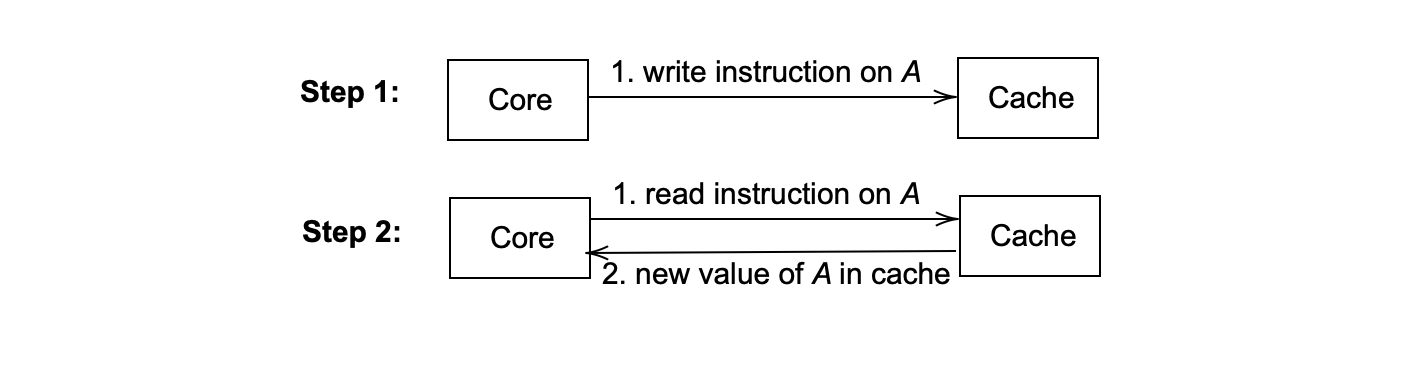
\includegraphics[width=1\textwidth,scale=0.5]{write_single_score_coherence.png}
        \caption{\label{fig:write_single_core} Write access on cache line}
\end{figure}

\section{Understanding of cache coherence in multiple cores}
To understanding coherence when we execute the same algorithm in parallel, suppose that we have 
a program $S$ running on 3 cores $C_1, C_2, C_3$ and accessing the shared memory address $L$.

\begin{figure}[h]
        \centering
        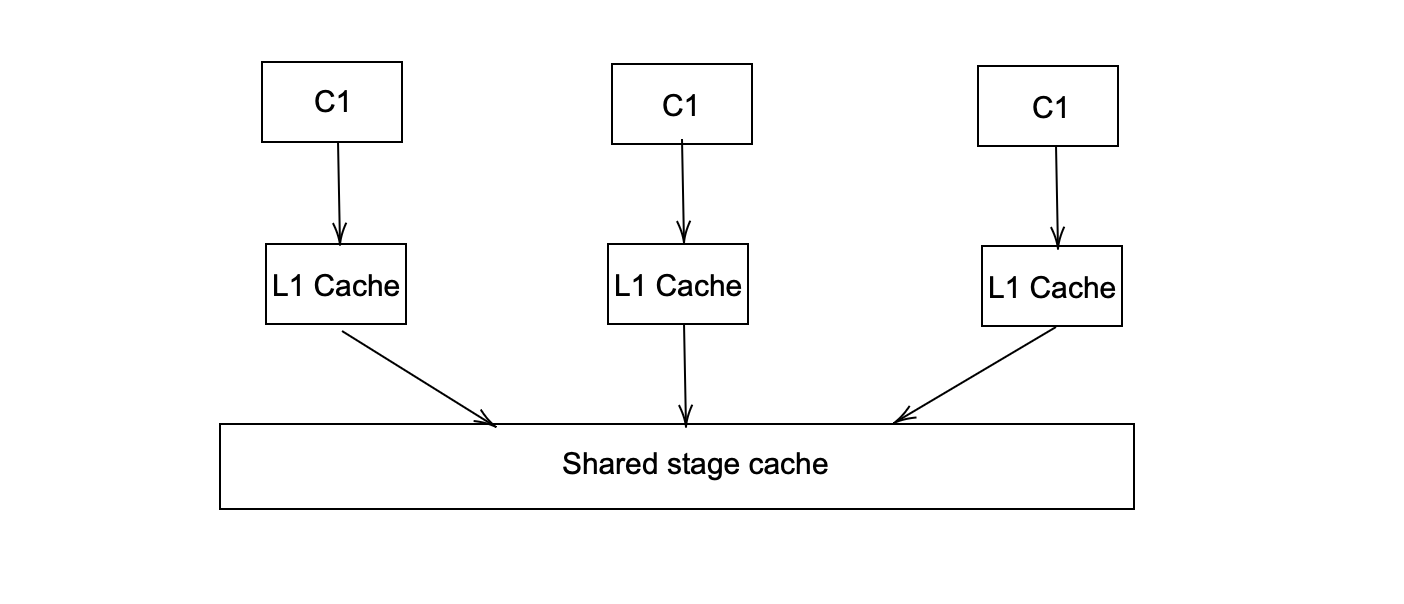
\includegraphics[width=0.7\textwidth,scale=0.5]{multicore_coherence_setup.png}
        \caption{\label{fig:multicore_setup} Parallel access which shared memory}
\end{figure}

Therefore, each core have to read data from address $L$ if their local cache is missing or dirty and some cores
update the value in shared stage memory. The process is similar to single core, but each core needs to communicate
to each other by transferring a message in interconnection network in order to keep the `last' write value to memory.
That means every time core $C_i$ where $i = 1,2,3$ updates the value in memory address $L$ the local cache of the rest 
will become dirty immediately which also means that the core need to inform to others that the value is being updated 
and fetch the value by read instruction. Now the problem begins that decrease the performance. Due to the message delay and latency
between interconnection network, the ordering of write and read disoriented as we need to guarantee that every time we read value
it must be the latest update across all cores. This is also called false sharing. One way to achieve coherency for accesses is to have the writing core wait for all caches
to receive the previous write value before sending a new write task which is called \textbf{an acknowledgement message (ACK)}.

\section{Coherence for Shared Memory in Parallel Execution}
As we explained in the previous section, the concept of coherence in single core applies to all cores when we run tasks
simultaneously on shared memory. A single core executes accesses to a single memory location with an order. When we add caches and multiple cores accessing the same memory locations,
everything does not seem to work out nicely. Caches allow cores to read values written by previous writer and all caches must be updated.
There are two invariants which define what is required for a parallel execution on memory accesses to be consistent which are 
\begin{enumerate}
        \item Single-Write-Multiple-Readers (SWMR): At any time, every memory location $L$  has either one core that may write and read $L$ (writer-reader period), or any number of cores that can only read $L$ (readers period) stated by \cite{hay2012mesif}.
        \item Data-Value: The value of a memory location is the previous value written by this core if this core is writing. Or it is the last value written by the previous writing core, 
                if there is no writer
\end{enumerate}
To clarify more, SWMR invariant guarantees that for each memory location at any time, there is either one writer who can also read location $L$ or many readers who can not write to memory.
The invariant is similar to how rust compiler handle concurrency with ownership. Next, Data-Value invariant states that value of read access
is either the last value written by the previous writing core (the previous writer-reader).

\section{Cache Coherence Protocols}
To understand cache coherence protocol, it is a set of rules that ensures that the data in different memories that share a common memory is kept consistent.
There are a few important components that we need to understand for cache coherence protocol in a multicore system. In particular, there are also two well-know categories of cache coherence protocols which are directories and snooping.
Snooping cache protocol distributes the coherence information around the system and make cache controllers responsible for maintaining information about copies of memory locations for which they have special privileges.
Directory-based cache protocol depends on a single place to store information about a cache line. each address is associated with a given location where the coherence information is maintained while the information may be distributed for difference addresses.

\subsection{System Components}
A core is a processing unit with a single thread of execution that executes some multi-threaded program consisting of multiple sequence of instructions, each core runs one sequence of instructions (\citealp*{hay2012mesif}).
Some instructions are memory operations which either read from memory locations or write to it. Each core handles memory operations using associated finite state machine (FSM) called cache controller which encodes the rules of cache coherence protocol designed to achieve coherence
as shown in figure \ref*{fig:system_component}.

\begin{figure}[h]
        \centering
        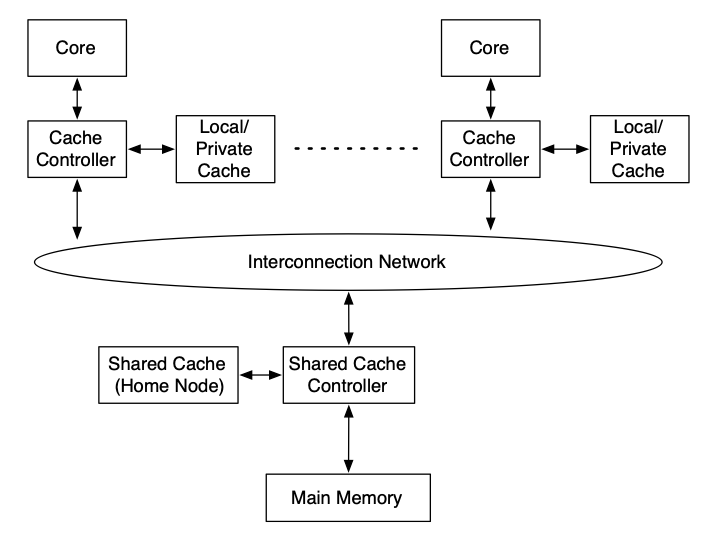
\includegraphics[width=0.6\textwidth,scale=0.5]{system_component.png}
        \caption{\label{fig:system_component} System component with cache controller and protocol provided by \citealp{hay2012mesif}}
\end{figure}
\newpage
Memory operation enables the local cache controller to check if the local cache has the correct permissions to service the memory operation from the cache. The permissions are encoded in cache states which helps to
satisfy the mentioned 2 invariants (SWMR and Data-Value). That means that if the location has the right permission, the memory operation hits in the cache and 
can be serviced by the local cache without communicating with other caches. Otherwise, the cache is missed adn the controller issue a memory request for the cache block requesting to write or read.

\subsection{Interconnection Network}
This component is the part that joins all local caches together in multiple cores adn the controller of each local cache. Network nodes can address other network nodes with virtual address to exchange messages and data inside a machine.
Also, the cache coherence protocol uses messages and send data through the interconnection network to service memory while ensuring that the system is consistent and write-read memory across all cores.
There are 3 different types of interconnection network with a different benefits and drawbacks.
\begin{enumerate}
        \item Totally-ordered: all nodes receive all messages in the same order.
        \item Point-to-Point: message sent between two nodes are delivered in order
        \item Unordered: no guarantee on the ordering of messages sent through them.
\end{enumerate}
In the real world, two main types are considered in most and current architecture which are
\begin{enumerate}
        \item Bus based interconnection: Nodes communicate over a shared medium which is a set of wires.
        \item Point-to-point interconnection: nodes are linked together directly into topology. A node can send message
                only yo nodes that they are linked together.
\end{enumerate}
With bus interconnection, it guarantees that the message and data are broadcasted with order with limit bandwidth which can cause bottleneck.
Point-to-point is more scalable as it has lower latency and higher bandwidth than bus interconnection.



\chapter{Existing Solution}
Recall that false sharing is caused when two CPUs what to access two different data in the same cache block because cache coherency prevents two CPUs from reading and wrtting in the the same cache block
, this creates an unessary wast of time since the two data they want to access are not from the same location.
A naive approch to solving this problem is to just get rid of cache coherence,
 but this will cause chaous when multiple processors are tring to read and write to the same data location known as data race. Therefore a good approch in reducing false sharing must not disterbe the perpos on having cache coherency in the fist place.

\section{Reducing False Sharing through Compile Time Data Transformations}

Instaed of altering the cache coherence protocal one way to reduce false sharing is by organizing the data in such a way that false sharing is less liking to occur.
In \citealp{jeremiassen1995reducing} suggest that this may be done by the compiler. Increasing the compilation time, but decreasing the running time.
For false sharing to not occur, data that are access by only one processors must be grouped togather in the same cahce block, and data that is shared by multiple processors with no processor locality do not share cache blocks.
By grouping data that are used by the same processor togather, it ensures that the probability of haveing two processors accessing the same cahce block is reduce greatly, which interns reduces false sharing.
To acomplish this \citealp*{jeremiassen1995reducing} have stated three techniques to reduce false sharing which are group and transpose, indirection, and pad and alingn.

\subsection*{Group and Transpose}
group and transpose works by crated vectors such that adjacent elements in a vector are accessed by different processors and then tranpose it.
If any processor's data is less than the cahce block size then it may be padded.
This is to ensure that no two processors share the same cache block.
Inaddition to reduceing false sharing, This transformation improves spatial locality,
which means that data that is access by the same processor are more liky to be in the same chahe block incresing the retrival time of some data.

\subsection*{Indirection}
When it is not posible to group data togather, we can acomplish something similar by using pointers or indirection. This is done by allocating an array of data areas that is going to be access by a specific prossor,
place shared data into them, and locates the share data with pointers that replace the values of the original data.

\subsection*{Pad and Align}
Another way of reducing false sharing is to use padding. This works by padding data that is going to be access by only one processor so that it completly fills the cache block. This makes it so that no other data can be place in the same cache block.
Although this method does reduce false sharing, it is not space efficient since the padded space can not be use to keep data.
Moreover, by haveing each data in it's own cache block it gradly reduces spatial locality.
In order to use this method effactively, it is best to pad data that are almost as large as the cache block or data that is risk of creating false sharing.


\begin{figure}[h]
        \centering
        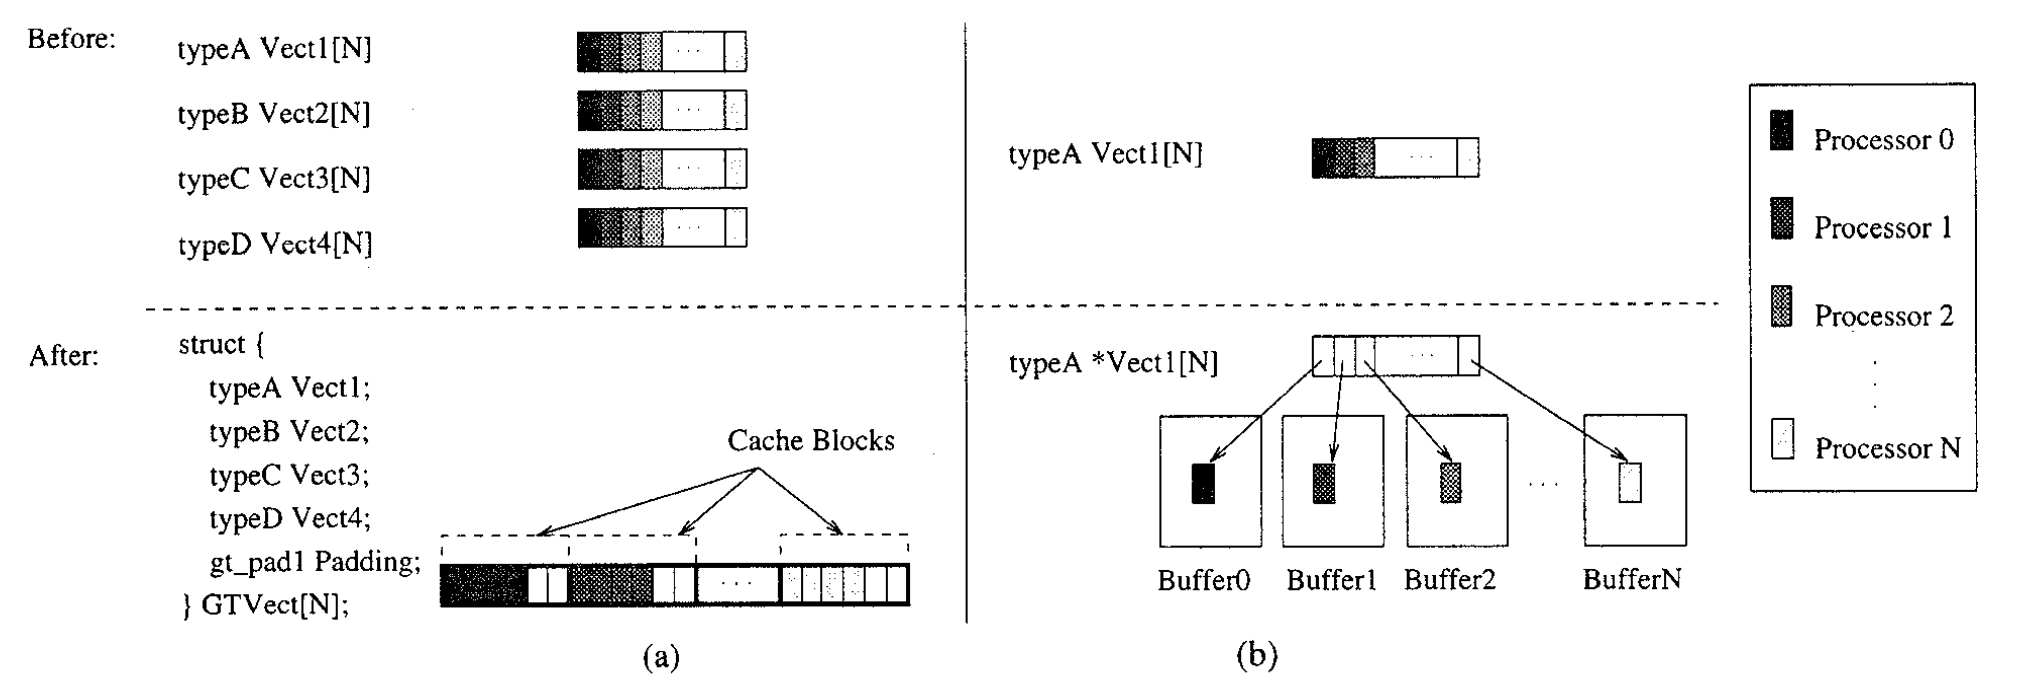
\includegraphics[width=1\textwidth,scale=0.5]{solutions.png}
        \caption{\label{fig:false_sharing_solutions} (a) group and transpose, (b) indirection}
\end{figure}

\subsection{Results}
\citealp*{jeremiassen1995reducing} have gien experimental results for the methods of reduceing false sharing on some known algorithms as in figure \ref*{fig:false_sharing_programs}. and the results are given in figure \ref*{fig:false_sharing_table}. 

    


\begin{figure}[h]
        \centering
        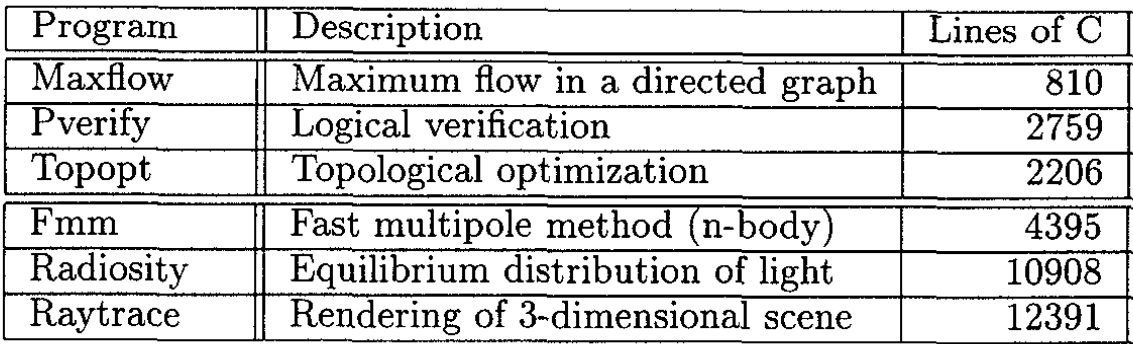
\includegraphics[width=1\textwidth,scale=0.5]{false-sharing_programs.png}
        \caption{\label{fig:false_sharing_programs} Programs that are tested with these methods.}
\end{figure}

\begin{figure}[h]
        \centering
        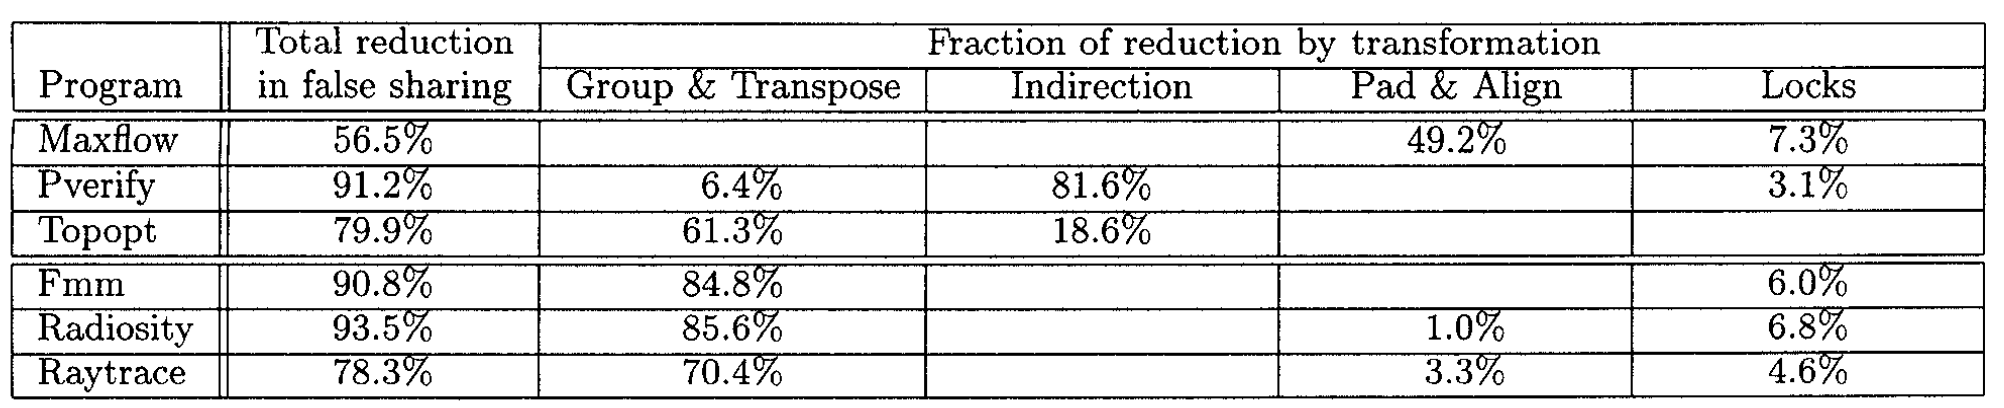
\includegraphics[width=1\textwidth,scale=0.5]{false-sharing_table.png}
        \caption{\label{fig:false_sharing_table} The false sharing miss rate reduction broken down by transformation. Numbers are averages over 8-256 byte cache}
\end{figure}



\chapter{Possible Solution}
\section{Adjustable Block Size Coherent Cache}

It is easy to see that the amount of false sharing proportional the cache block size. As, the cache block size gets bigger the chances of false sharing will increas due to the fact that a bigger block size can store more data, thus more liky that two processors that two different data from the size cache block, and vice versa.
False sharing can be reduce for large block size by using padding as stated earlier, but this comes with a disadvantage of haveing unusable space.
To fix this problem we suggest to use an adjustable block size coherent cache as stated in \citealp*{dubnicki1992adjustable}.
\citealp*{dubnicki1992adjustable} stated a way of adjusting the block size by merging chahe blocks to increas it's size and spliting cache block to decres it's size.
This may eleminate the space problem from padding, but the trade off of spatial locality still remains. 

\section{Group and Transpose with Adjustable Block Size Coherent Cache}\label{sec:cobination}
To eleminate the spatial locality problem that adjacenting the block size may have in reduceing
fase sharing. It is better to use this method in conjunction with other methods of reducing false sharing such as, the group and tranpose method that was stated earlier. Recall that grop and tranpose reduces false sharing by grouping data that are used by the same processor togather and pad the data that dose not fill the cache block. We can improves both false sharing and spatial locality by grouping all the data that is going to be access by the same process togather and putting in the smallest cache block that can contain the data group.
This can be taken one step further by also padding the data group if it doesn't fill the cache block.




% \citet{Jacobson1999Towards} states that \ldots

\bibliography{reference}
\bibliographystyle{plainnat}
\end{document}
